\documentclass[svgnames,11pt]{beamer}
\input{/home/tof/Documents/Cozy/latex-include/preambule_commun.tex}
\input{/home/tof/Documents/Cozy/latex-include/preambule_beamer.tex}
%\usepackage{pgfpages} \setbeameroption{show notes on second screen=left}
\author[]{Christophe Viroulaud}
\title{Portes logiques}
\date{\framebox{\textbf{ArchMat 05}}}
%\logo{}
\institute{Première - NSI}

\begin{document}
\begin{frame}
    \titlepage
\end{frame}
\begin{frame}
    \frametitle{}

    Un ordinateur effectue des calculs en binaire. En pratique il ne \emph{voit} pas des 0 et des 1 mais des signaux électriques.

\end{frame}
\begin{frame}
    \frametitle{}

    \begin{framed}
        \centering Comment effectuer des opérations complexes avec un signal binaire?
    \end{framed}

\end{frame}
\section{Contexte historique}
\begin{frame}
    \frametitle{Contexte historique}
    \begin{center}
        \centering
        \includegraphics[width=4cm]{ressources/Metier_jacquard.jpg}
        \captionof{figure}{\centering \textbf{1801: }Métier à tisser du lyonnais Joseph Marie Jacquard. Premier système mécanique programmable avec cartes perforées. }
        \label{IMG}
    \end{center}


\end{frame}
\begin{frame}
    \frametitle{}

    \begin{center}
        \centering
        \includegraphics[width=8cm]{ressources/babbage.jpeg}
        \captionof{figure}{\centering \textbf{1834: }Machine analytique de Babbage.}
        \label{IMG}
    \end{center}
    \note{s'inspire de métier Jacquard}
\end{frame}
\begin{frame}
    \frametitle{}

    \begin{center}
        \centering
        \includegraphics[width=5cm]{ressources/George_Boole_color.jpg}
        \captionof{figure}{\centering \textbf{1847: }Georges Boole développe une nouvelle forme de logique, à la fois symbolique et mathématique.}
        \label{IMG}
    \end{center}

\end{frame}
\begin{frame}
    \frametitle{}

    \begin{center}
        \centering
        \includegraphics[width=5cm]{ressources/Diode_flemming.PNG}
        \captionof{figure}{\centering \textbf{1904: }Flemming invente la diode à vide. En 1906, De Forest ajoute une troisième électrode (la grille de contrôle): naissance de la triode.}
        \label{IMG}
    \end{center}
    \note{tube à vide ou tube électronique}
\end{frame}
\begin{frame}
    \frametitle{}

    \begin{center}
        \centering
        \includegraphics[width=8cm]{ressources/Eniac.jpg}
        \captionof{figure}{\centering \textbf{1945: } ENIAC (Electronic Numerical Integrator And Computer) premier calculateur entièrement électronique}
        \label{IMG}
    \end{center}
    \note[item]{30 tonnes}
    \note[item]{utilise tubes à vide}
\end{frame}
\begin{frame}
    \frametitle{}

    \begin{center}
        \centering
        \includegraphics[width=8cm]{ressources/transistor.jpg}
        \captionof{figure}{\centering \textbf{1947: }Invention du transistor par Bradley, Shockley et Brattain}
        \label{IMG}
    \end{center}
    \note{remplace petit à petit tubes à vide}
\end{frame}
\begin{frame}
    \frametitle{}

    \begin{center}
        \centering
        \includegraphics[width=6cm]{ressources/transistor-img.jpg}
        \captionof{figure}{\centering \textbf{années 50: }Le transistor devient plus fiable et plus petit.}
        \label{IMG}
    \end{center}

\end{frame}
\begin{frame}
    \frametitle{}

    \begin{center}
        \centering
        \includegraphics[width=6cm]{ressources/circuitintegre.JPG}
        \captionof{figure}{\centering \textbf{1958: }Jack Kilby invente le circuit intégré qui regroupe plusieurs transistors.}
        \label{IMG}
    \end{center}

\end{frame}
\begin{frame}
    \frametitle{}

    \begin{center}
        \centering
        \includegraphics[width=8cm]{ressources/Intel_C4004.jpg}
        \captionof{figure}{\centering \textbf{1971: }Les circuits intégrés remplace peu à peu les transistors. Le 4004 d'Intel est le premier microprocesseur commercialisé.}
        \label{IMG}
    \end{center}
    \note[item]{2300 transistors}
    \note[item]{60000 opérations par seconde}
\end{frame}
\begin{frame}
    \frametitle{}

    \begin{center}
        \centering
        \includegraphics[width=6cm]{ressources/raw.jpeg}
        \captionof{figure}{\centering \textbf{2008: }la carte graphique GT200 de Nvidia atteint 1 milliard de transistors sur un seul composant.}
        \label{IMG}
    \end{center}
    \note[item]{aujourd'hui, entre 20 et 30 milliards de transistors sur CPU}
\end{frame}
\section{Produire un signal binaire}
\subsection{Le transistor}
\begin{frame}
    \frametitle{Signal binaire - le transistor}

    \begin{center}
        \centering
        \includegraphics[width=7cm]{ressources/transistor-schema.png}
        \captionof{figure}{\centering Un transistor se comporte comme un interrupteur qui laisse ou non passer le courant sur le principe
            du tout ou rien.}
        \label{IMG}
    \end{center}

\end{frame}
\begin{frame}
    \frametitle{}
    \begin{center}
        \includegraphics[width=5cm]{ressources/transistor-schema.png}
    \end{center}

    Broche B:
    \begin{itemize}
        \item sous tension, elle laisse passer le courant entre la broche E est la masse,
        \item sous tension basse, la broche E reste sous tension haute.
    \end{itemize}
\end{frame}
\begin{frame}
    \frametitle{}


    \begin{aretenir}[]
        Un transistor laisse passer en sortie un courant ou non selon un ordre en entrée. On obtient \textbf{un signal binaire}.
    \end{aretenir}

\end{frame}
\subsection{Première porte logique : NOT}
\begin{frame}
    \frametitle{Première porte logique : NOT}

    \begin{aretenir}[]
        Une porte logique est une fonction qui accepte un ou plusieurs bits en entrée et qui produit un bit
        en sortie.
    \end{aretenir}

\end{frame}
\begin{frame}
    \frametitle{}
    Un transistor permet de réaliser une opération élémentaire:
    \begin{itemize}
        \item un courant en entrée $\rightarrow$ pas de courant en sortie,
        \item pas de courant en entrée $\rightarrow$ un courant en sortie,
    \end{itemize}


\end{frame}
\begin{frame}
    \frametitle{NOT}

    \begin{center}
        \begin{tabular}{cc}
            \includegraphics[width=5cm]{ressources/not-us.png}
                              &
            \includegraphics[width=5cm]{ressources/not-eu.png} \\
            Symbole américain & Symbole européen               \\
        \end{tabular}
    \end{center}

\end{frame}
\begin{frame}
    \frametitle{}
    \begin{aretenir}[]
        On construit \textbf{la table de vérité} de la porte logique.
    \end{aretenir}
    \begin{center}
        \begin{tabular}{|c|c|}
            \hline
            Entrée & Sortie \\
            \hline
            1      & 0      \\
            \hline
            0      & 1      \\
            \hline
        \end{tabular}
        \captionof{table}{Fonction NOT}
    \end{center}

\end{frame}
\section{Combinaisons de transistors}
\subsection{Porte NOT OR}
\begin{frame}
    \frametitle{Porte NOT OR}
    \begin{center}
        \centering
        \includegraphics[width=7cm]{ressources/schema-nor.png}
        \captionof{figure}{Deux transistors en parallèle}
        \label{IMG}
    \end{center}

    \begin{activite}
        Établir la table de vérité de la combinaison de deux transistors en parallèle.
    \end{activite}
\end{frame}
\begin{frame}
    \frametitle{}

    \begin{center}
        \begin{tabular}{|c|c|c|}
            \hline
            E1 & E2 & S \\
            \hline
            0  & 0  & 1 \\
            \hline
            0  & 1  & 0 \\
            \hline
            1  & 0  & 0 \\
            \hline
            1  & 1  & 0 \\
            \hline
        \end{tabular}
        \captionof{table}{Fonction NOT OR (NOR)}
    \end{center}

\end{frame}
\begin{frame}
    \frametitle{NOR}

    \begin{center}
        \begin{tabular}{cc}
            \includegraphics[width=5cm]{ressources/not-or-us.png}
                              &
            \includegraphics[width=5cm]{ressources/not-or-eu.png} \\
            Symbole américain & Symbole européen                  \\
        \end{tabular}
    \end{center}

\end{frame}
\subsection{Porte NOT AND}
\begin{frame}
    \frametitle{Porte NOT AND}
    \begin{center}
        \centering
        \includegraphics[width=3cm]{ressources/schema-nand.png}
        \captionof{figure}{Deux transistors en série}
        \label{IMG}
    \end{center}


\end{frame}
\begin{frame}
    \frametitle{}

    \begin{center}
        \begin{tabular}{|c|c|c|}
            \hline
            E1 & E2 & S \\
            \hline
            0  & 0  & 1 \\
            \hline
            0  & 1  & 1 \\
            \hline
            1  & 0  & 1 \\
            \hline
            1  & 1  & 0 \\
            \hline
        \end{tabular}
        \captionof{table}{Fonction NOT AND (NAND)}
    \end{center}

\end{frame}
\begin{frame}
    \frametitle{NAND}

    \begin{center}
        \begin{tabular}{cc}
            \includegraphics[width=5cm]{ressources/not-and-us.png}
                              &
            \includegraphics[width=5cm]{ressources/not-and-eu.png} \\
            Symbole américain & Symbole européen                   \\
        \end{tabular}
    \end{center}

\end{frame}
\section{Combinaisons de portes logiques}
\subsection{Porte NOT}
\begin{frame}
    \frametitle{Porte NOT}

    \begin{aretenir}[]
        En combinant plusieurs blocs élémentaires, on peut construire d'autres portes logiques.
    \end{aretenir}
    Il est possible de fabriquer une porte NOT en reliant les 2 entrées d’une porte NAND.
    \begin{center}
        \centering
        \includegraphics[width=4cm]{ressources/not-from-nand.png}
        \captionof{figure}{Reconstruire une porte NOT}
        \label{IMG}
    \end{center}
\end{frame}
\subsection{Porte OR}
\begin{frame}
    \frametitle{Porte OR}

    \begin{center}
        \centering
        \includegraphics[width=8cm]{ressources/or-from-nand.png}
        \captionof{figure}{Combinaisons de portes NAND: porte OR}
    \end{center}
    \begin{activite}
        Construire la table de vérité de la porte OR.
    \end{activite}
\end{frame}
\begin{frame}
    \frametitle{}
    \begin{center}
        \begin{tabular}{|c|c|c|}
            \hline
            A & B & out \\
            \hline
            0 & 0 & 0   \\
            \hline
            0 & 1 & 1   \\
            \hline
            1 & 0 & 1   \\
            \hline
            1 & 1 & 1   \\
            \hline
        \end{tabular}
        \captionof{table}{Fonction OR}
    \end{center}

\end{frame}
\begin{frame}
    \frametitle{OR}
    \begin{tabular}{cc}
        \includegraphics[width=5cm]{ressources/or-us.png}
                          &
        \includegraphics[width=5cm]{ressources/or-eu.png}
        \\
        Symbole américain & Symbole européen \\
    \end{tabular}


\end{frame}
\subsection{Porte AND}
\begin{frame}
    \frametitle{Porte AND}

    \begin{center}
        \centering
        \includegraphics[width=8cm]{ressources/and-from-nor.png}
        \captionof{figure}{Combinaisons de portes NOR: porte AND}
    \end{center}
    \begin{activite}
        Construire la table de vérité de la porte AND.
    \end{activite}
\end{frame}
\begin{frame}
    \frametitle{}
    \begin{center}
        \begin{tabular}{|c|c|c|}
            \hline
            A & B & out \\
            \hline
            0 & 0 & 0   \\
            \hline
            0 & 1 & 0   \\
            \hline
            1 & 0 & 0   \\
            \hline
            1 & 1 & 1   \\
            \hline
        \end{tabular}
        \captionof{table}{Fonction AND}
    \end{center}

\end{frame}
\begin{frame}
    \frametitle{AND}
    \begin{tabular}{cc}
        \includegraphics[width=5cm]{ressources/and-us.png}
                          &
        \includegraphics[width=5cm]{ressources/and-eu.png}
        \\
        Symbole américain & Symbole européen \\
    \end{tabular}


\end{frame}
\subsection{Porte XOR}
\begin{frame}
    \frametitle{Porte XOR}

    \begin{aretenir}[]
    Le \textbf{ou exclusif} donne un résultat 1  quand une des deux entrées seulement est à 1.
    \end{aretenir}
\begin{activite}
Construire la table de vérité du \textbf{ou exclusif}.
\end{activite}
\end{frame}
\begin{frame}
    \frametitle{}

    \begin{center}
        \begin{tabular}{|c|c|c|}
            \hline
            A & B & out \\
            \hline
            0 & 0 & 0   \\
            \hline
            0 & 1 & 1   \\
            \hline
            1 & 0 & 1   \\
            \hline
            1 & 1 & 0   \\
            \hline
        \end{tabular}
        \captionof{table}{Fonction XOR}
    \end{center}

\end{frame}
\begin{frame}
    \frametitle{XOR}
    \begin{tabular}{cc}
        \includegraphics[width=5cm]{ressources/xor-us.png}
                          &
        \includegraphics[width=5cm]{ressources/xor-eu.png}
        \\
        Symbole américain & Symbole européen \\
    \end{tabular}


\end{frame}
\end{document}